\documentclass[a4paper, 12pt]{article}
\usepackage[slovene]{babel}
\usepackage[utf8]{inputenc}
\usepackage{url}
\usepackage{hyperref}
\usepackage{listings}
\usepackage{amsmath}
\usepackage{amssymb}
\usepackage{float}
\usepackage{subcaption}
\usepackage{eurosym}
\usepackage{graphicx}
\graphicspath{ {C:/Users/dmoho/Documents/FRI/2_letnik_1_semester/VS/slike/} }

\begin{document}

\title{Najemnine v Ljubljani}
\author{Domen Mohorčič}
\maketitle

\section{Uvod}

Ko se povprečen Slovenec odseli od staršev v svoje stanovanje, je star 28,2
leti (\href{https://www.stat.si/statweb/News/Index/7570}{stat.si}). Pred
izselitvijo pa si mora stanovanje poiskati. Po navadi ljudje pri izbiri
stanovanja gledajo na to, ali jim je stanovanje všeč in ali se jim zdi cena
ustrezna stanovanju. Od česa pa sploh je odvisna cena stanovanja? Friškovec
(2010)[1] ugotavlja, da je oglaševalska cena stanovanja
pozitivno odvisna od površine, števila kopalnic in ali gre za mansardno
stanovanje, negativno pa predvsem od višine nadstropja. Repič (2014)[2] pa je
v magistrski nalogi pokazala, da je prodajna cena stanovanja pozitivno odvisna
od prisotnosti dvigala, parkirnega mesta, opremljenosti stanovanja, bližine
središča Ljubljane in števila sob v stanovanju, negativno pa na ceno vplivajo
starost stanovanja, površina in trajanje, ko je nepremičnina na voljo za
prodajo.

V Sloveniji v najemniških stanovanjih živi le 2,4
gospodinjstev (\href{https://cekin.si/nepremicnine/trnova-pot-do-lastnega-doma-zakaj-mora-biti-tako.html}{cekin.si}).
Kljub temu je trg najema nepremičnin kar velik, še posebej v Ljubljani (na
nepremicnine.net je od 1500 oglasov za najem, od tega kar 1000 v Ljubljani),
kjer pa so najbolj zaželjeni študentje ali posamezniki. Nikjer pa nisem
zasledil raziskave, ki bi ugotavljala, kaj vpliva na ceno najema.

Namen seminarske naloge je ugotoviti, kateri dejavniki najbolj vplivajo na ceno
najemnin v Ljubljanskima predeloma Vič in Rudnik.

\section{Podatki}

Podatke sem pridobil iz slovenske spletne strani
\href{https://www.nepremicnine.net}{nepremicnine.net} dne 8.8.2020.
Iskal sem stanovanja v Ljubljani v predelih Vič in Rudnik.
Pri pregledovanju oglasov sem se osredotočil na naslednje podatke:
nadstropje, v katerem se stanovanje nahaja, število vseh nadstropij v zgradbi,
leto gradnje stavbe, leto prenove stanovanja, število sob v stanovanju,
ali ima stanovanje shrambo/klet, ali je stanovanje opremljeno, število
pripadajočih parkirišč, velikost bivalne površine, zunanje površine
(balkon, vrt, \dots), mesečni stroški bivanja in cena najema. Ker pa sem hotel
ugotoviti, ali na ceno najema vpliva tudi lokacija stanovanja, sem poiskal še
oddaljenost do središča Ljubljane (v mojem primeru Prešernov trg). Na prej
omenjeni spletni strani pa v večini primerov ni napisanega točnega naslova,
zato sem iskal samo približne lokacije (ulica ali naselje).

Pri določanju razdalje sem si pomagal z orodjem
\href{https://www.distance.to/}{distance.to}. Za analizo podatkov sem uporabil
program \href{https://rstudio.com/}{RStudio}.

\subsection{Opis spremenljivk}

Zbrane podatke sem označil z naslednjimi spremenljivkami:
\begin{table}[h]
\begin{center}
\caption{Tabela spremenljivk in njihov opis}
\label{table:1}
\begin{tabular}{ c|c}
	spremenljivka & opis \\
	\hline
	\hline
	nadstropje & V katerem nadstropju se stanovanje nahaja \\
	\hline
	vsaNadstropja & Število vseh nadstropij v stavbi \\
	\hline
	letoGradnje & Leto, v katerem je bilo stanovanje zgrajeno \\
	\hline
	letoPrenove & Leto, v katerem je bilo stanovanje prenovljeno \\
	\hline
	stSob & Število sob v stanovanju \\
	\hline
	stParkirisc & Število parkirnih mest, ki pripadajo stanovanju \\
	\hline
	parkirisce & Ali stanovanju pripada lastno parkirišče \\
	\hline
	opremljenost & Kako je stanovanje opremljeno (polno, delno ali nič) \\
	\hline
	shramba & Ali stanovanju pripada zunanja soba za shranjevanje \\
	\hline
	zunanjePovrsine & Vsota zunanjih površin stanovanja \\
	\hline
	povrsina & Velikost bivalne površine v stanovanju \\
	\hline
	oddaljenost & Oddaljenost stanovanja od Prešernovega trga \\
	\hline
	cena & Cena mesečne najemnine stanovanja \\
	\hline
	stroski & Cena mesečnih stroškov bivanja \\
	\hline
	skCena & Seštevek cene in mesečnih stroškov bivanja \\
\end{tabular}
\end{center}
\end{table}

Za model napovedi mesečne najemnine sem izbral spremenljivke $ skCena $,
$ parkirisce $, $ povrsina $, $ letoGradnje $ in
$ oddaljenost $. $ skCena $ je odvisna spremenljivka, ostale štiri pa
so neodvisne.

Spremenljivko $ letoPrenove $ sem odstranil iz modela, ker za večino
stanovanj podatka nisem našel. $ nadstropje $ in $ vsaNadstropja $
sem izvzel, ker pri pregledu oglasov nisem dobil občutka, da bi ti dve
spremenljivki pomembno vplivali na ceno najemnine. Spremenljivko
$ opremljenost $ sem odstranil, ker je bilo $ 89.3\% $ stanovanj
opremljenih in tako ni bilo dovolj raznolikosti. Pri pregledu korelacijske
matrike sem ugotovil, da sta spremenljivki $ povrsina $ in
$ stSob $ povezani s korelacijskim koeficientom $ 0.811 $ zato sem obdržal
spremenljivko $ povrsina $. Namesto $ stParkirisc $ sem uporabil
spremenljivko $ parkirisce $, saj je tako bolje predstavljeno, ali ga
stanovanje ima. Spremenljivko $ zunanjePovrsine $ pa sem  odstranil iz
modela, ker je imela večina stanovanj samo balkon, redko pa so se pojavili
velikimi vrtovi.

\subsection{Analiza podatkov}

Izmed petih spremenljivk so $ letoGradnje $, $ povrsina $,
$ oddaljenost $ in $ skCena $ zvezne, $ parkirisce $ pa je
diskretna. Zbral sem podatke o 120 različnih stanovanjih ($ N = 120 $).

Za vsako zvezno spremenljivko sem izračunal povprečje, standardni odklon,
mediano absolutnih odstopanj od mediane, asimetričnost in sploščenost.

Asimetričnost (skewness) nam pove, kako asimetrični so podatki. Negativna
vrednost pove, da je rep podatkov na levi (večina podatkov je na desni stran
grafa) in obratno. Na grafu se to vidi kot v katero smer so podatki razvlečeni.
Vrednost $ 0 $ nam pove, da so podatki porazdeljeni simetrično, $ >0 $ pove, da
so podatki razvlečeni v desno, $ <0 $ pa da so razvlečeni v levo.

Sploščenost (kurtosis) nam pove, kako močni so repi podatkov. Pozitivna
vrednost pove, da so repi dobro zastopani in graf izgleda bolj ploščato.
Negativna vrednost pove, da so repi slabo zastopani in graf izgleda zelo
špičast.

V tabeli so predstavljene prej omenjene lastnosti zveznih spremenljivk:
minimum (min), maksimum (max), povprečje (avg), mediana (median),
standardni odklon (sd), mediana absolutnih odstopanj od mediane (MAD), test
asimetričnosti (skew) in test sploščenosti (kurt):
\begin{table}[H]
\begin{center}
\caption{Tabela lastnosti spremenljivk}
\label{table:2}
\begin{tabular}{ c|cccccccc }
	& min & max & avg & sd & median & MAD & skew & kurt \\
	\hline
	letoGradnje & 1895 & 2020 & 1984.81 & 29.72 & 1995 & 25.20 & -1.14 & 0.81 \\
	povrsina & 10 & 207.90 & 68.92 & 39.96 & 65 & 37.06 & 0.67 & 0.23 \\
	oddaljenost & 0.89 & 5.07 & 2.51 & 1.01 & 2.22 & 0.90 & 0.69 & -0.29 \\
	skCena & 160 & 3700 & 945.86 & 706.03 & 800 & 308.38 & 2.19 & 5.29 \\
\end{tabular}
\end{center}
\end{table}

Ker pa se vrednosti testa asimetričnosti in sploščenosti razlikujejo od $ 0 $,
to kaže na nenormalno porazdelitev, in tako nam vrednosti o povprečju ali
standardnem odklonu povesta bolj malo. Veliko bolj si lahko pomagamo z mediano
in MAD, saj nam podatka data veliko boljši občutek o tem, kakšni so podatki.
Naredil sem še test normalnosti z ukazom {\sf shapiro.test()} (Shapiro-Wilk)
in test simetričnosti z {\sf symmetry.test()} (MGG):

\begin{table}[H]
\begin{center}
\caption{Tabela rezultatov testa normalnosti in simetrije}
\label{table:3}
\begin{tabular}{ c|cc|cc }
	& \multicolumn{2}{c}{Shapiro-Wilk} & \multicolumn{2}{c}{MGG} \\
	& w value & p value & Test statistics & p value \\
	\hline
	letoGradnje &  0.88384 & 3.184e-08 & -5.1319 & $<$2.2e-16 \\
	povrsina & 0.95714 & 0.0007503 & 1.4438 & 0.15 \\
	oddaljenost & 0.93178 & 1.244e-05 & 4.4071 & $<$2.2e-16 \\
	skCena & 0.75813 & 8.857e-13 & 3.9694 & $<$2.2e-16 \\
\end{tabular}
\end{center}
\end{table}

Shapiro-Wilk-ov test testira ničelno hipotezo, da je spremenljivka normalno
porazdeljena, proti alternativni hipotezi, da ni. Ničelno hipotezo sprejme, če
je p vrednost (p value) večja od 0,05. V našem primeru ima najvišjo p vrednost
spremenljivka $ povrsina $, vendar je še vedno pod mejo sprejetja. Nobena
spremenljivka tako ni normalno porazdeljena.

MGG (Miao, Gel, and Gastwirth) test simetričnosti pa testira hipotezo, da
je naš vzorec simetričen proti alternativni hipotezi, da vzorec ni simetričen.
Vse spremenljivke razen $ povrsina $ imajo p vrednost testa zelo majhno,
zato so nesimetrične. Spremenljivka $ povrsina $ pa je po MGG testu simetrično
porazdeljena. Na njenem grafu pa se vidi, da je bolj na meji simetrije.

Tudi ko pogledamo histograme na sliki \ref{figure:1}, vidimo, da ni nobena
spremenljivka normalno porazdeljena ali simetrična. Najbližje normalni
porazdelitvi je $ povrsina $, vendar je nagnjena v levo. Na grafu leta
gradnje \ref{figure:1a} se vidi, da je večina najemniških stanovanj novejših.
Ker je mediana 1995, je polovica stanovanj mlajših od 25 let. Veliko stanovanj
je še iz leta 1960 naprej, starejših pa je že lezo malo. Površina stanovanj na
grafu \ref{figure:1b} je približno simetrično porazdeljena, vseeno pa je več
manjših stanovanj. Redka stanovanja so zelo velika, večina stanovanj ima
površino do $150 m^{2}$ Oddaljenost od središča Ljubljane na grafu
\ref{figure:1c} je skoraj linearna z izjemo večine stanovanj na razdalji 2 km.
Zelo redka so tudi stanovanja skoraj v središču ali že izven Ljubljane.
Skupna cena mesečne najemnine na grafu \ref{figure:1d} pa ima večino podatkov
manj od 1000€ na mesec. Stanovanja z najemninami 2000€ ali več pa so stanovanja
tipa penthouse in so bolj luksuzna ter redkejša na trgu.

\begin{figure}[H]
\begin{subfigure}{0.5\textwidth}
	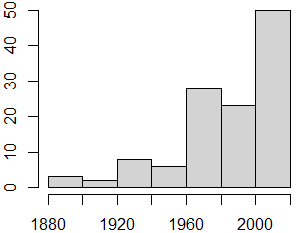
\includegraphics[width=6cm]{letoGradnje_hist.png}
	\caption{Leto gradnje}
	\label{figure:1a}
\end{subfigure}
\begin{subfigure}{0.5\textwidth}
	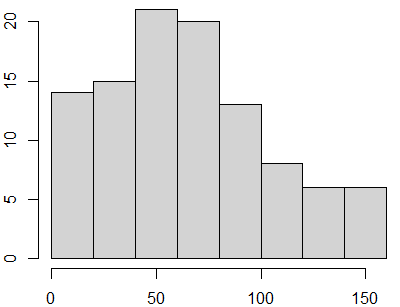
\includegraphics[width=6cm]{povrsina_hist.png}
	\caption{Povrsina}
	\label{figure:1b}
\end{subfigure}

\begin{subfigure}{0.5\textwidth}
	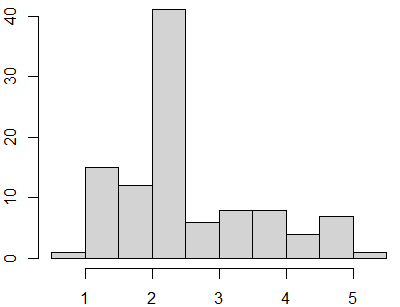
\includegraphics[width=6cm]{oddaljenost_hist.png}
	\caption{Oddaljenost}
	\label{figure:1c}
\end{subfigure}
\begin{subfigure}{0.5\textwidth}
	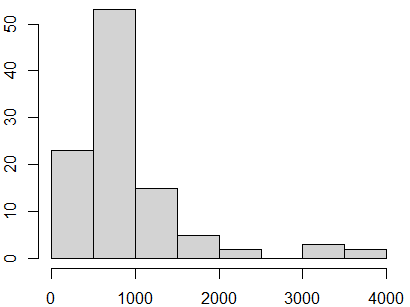
\includegraphics[width=6cm]{skCena_hist.png}
	\caption{Skupna cena}
	\label{figure:1d}
\end{subfigure}
\caption{Histogrami zveznih spremenljivk}
\label{figure:1}
\end{figure}

Spremenljivka $ parkirisce $ je diskretna, zato jo lahko predstavimo z
vzorčnim deležem:

\begin{center}
\begin{tabular}{ c|cc }
	& da & ne \\
	\hline
	parkirisce & 0.55 & 0.45 \\
\end{tabular}
\end{center}

\section{Večkratna regresija}

Linearna regresija je analiza, pri kateri ugotavljamo funkcijsko zvezo med
dvema spremenljivkama ($ X $ in $ Y $), pri večkratni regresiji pa funkcijsko
zvezo med več spremenljivkami, kjer je ena odvisna ($ Y $), ostale pa neodvisne.
Cilj analize je najti linearno funkcijo, ki najbolje opiše obnašanje odvisne
spremenljivke v odvisnosti od ostalih spremenljivk. Pri tem pa mora veljati
nekaj predpostavk regresijskega modela:
\begin{enumerate}
	\item $ Y $ je lienarna funkcija neodvisnih spremenljivk $ X_{1}, X_{2}, \dots $
	\item Napake $ \epsilon_{i} $ so med sabo neodvisne,
	\item Napake $ \epsilon_{i} $ imajo konstantno varianco,
	\item Napake $ \epsilon_{i} $ so normalno porazdeljene.
\end{enumerate}

\subsection{Koeficienti korelacije}

Pri modelu večkratne regresije je najprej potrebno preveriti, kako so
neodvisne spremenljivke povezane med sabo. Če so povezane preveč, lahko z neko
spremenljivko opišemo drugo, in tako iz druge ne izvemo nič novega ali pa zelo
malo o odvisni spremenljivki.

Pearsonov koeficient korelacije meri linearno odvisnost med dvema
spremenljivkama ima vrednost med $ -1 $ in $ 1 $. Če ima vrednost blizu
$ 1 $, sta spremenljivki pozitivno povezani, če pa ima vrednost blizu $ -1 $,
sta negativno povezani. Če vrednost znaša $ 0 $, spremenljivki nista
povezani. Povezanost pa se drugče opisuje kot šibko, srednjo in močno glede na
absolutno velikost koeficienta in pozitivno ali negativno glede na predznak.
V spodnji tabeli so predstavljeni pearsonovi koeficienti korelacije za zvezne
spremenljivke:
\begin{table}[H]
\begin{center}
\caption{Pearsonovi linearni koeficienti korelacije}
\begin{tabular}{ c|cccc }
	& letoGradnje & povrsina & oddaljenost & skCena \\
	\hline
	letoGradnje & 1.000 & 0.081 & 0.267 & 0.176 \\
	povrsina & 0.081 & 1.000 & -0.070 & 0.846 \\
	oddaljenost & 0.267 & -0.070 & 1.000 & -0.131 \\
	skCena & 0.176 & 0.846 & -0.131 & 1.000 \\
\end{tabular}
\end{center}
\end{table}

Neodvisne spremenljivke $ letoGradnje $, $ povrsina $ in
$ oddaljenost $ imajo medsebojne koeficiente skoraj $ 0 $ z izjemo
$ letoGradnje $ in $ oddaljenost $, ki imata pozitiven koeficient
$ 0.267 $. Spremenljivki sta pozitivno šibko povezani, kar pomeni, da se
novejša stanovanja nahajajo malo bolj izven središča Ljubljane. Vidimo lahko
tudi, da imata spremenljivki $ povrsina $ in $ skCena $ pearsonov linearni
koeficient $ 0,846 $, kar nakazuje na močno linerano odvisnot. Iz tega lahko
sklepamo, da je mesečna najemnina stanovanj zelo odvisna od površine le tega.

Na sliki \ref{figure:2} vidimo, kako so posamezne spremenljivke povezane med
sabo. Iz grafov med spremenljivkami $ letoGradnje, povrsina $ in $ oddaljenost $
se ne vidi nobene očitne povezanosti, kljub temu da sta $ letoGradnje $ in
$ oddaljenost $ šibko povezani. Najbolj opazna odvisnost je med $ povrsina $ in
$ skCena $, ki izgleda zelo linearno z izjemo nekaj točk. To še dodatno
potrjuje našo ugotovitev o tem, da sta najemnina in površina stanovanja
povezani.

\begin{figure}[H]
	\centering
	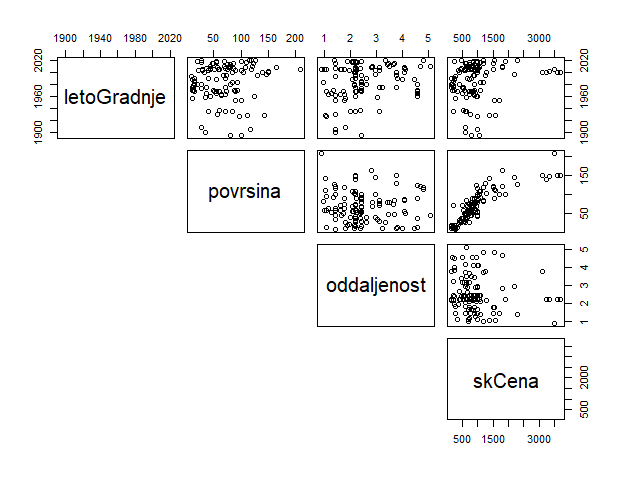
\includegraphics[width=13cm]{pairs.png}
	\caption{Grafični prikaz povezanosti spremenljivk}
	\label{figure:2}
\end{figure}

\subsection{Večkratna regresija}

Neodvisne spremenljivke našega modeal so $ letoGradnje, povrsina, oddaljenost $
in $ parkirisce $. Odvisna spremenljivka je $ skCena $. Funkcija našega
opisnega modela bo imela naslednjo obliko:
\begin{equation}
	skCena = a+b*letoGradnje+c*povrsina+d*oddaljenost+e*parkirisce+\epsilon
\end{equation}

$ b, c, d $ in $ e $ so koeficienti posameznih neodvisnih spremenljivk. $ a $
predstavlja začetno vrednost, sam po sebi pa nima smisla (stanovanje z $ 0 $ v
pri vseh neodvisnih spremenljivkah bi imelo $ a $ mesečne najemnine, tako
stanovanje pa ne obstaja). $ \epsilon $ predstavlja odstopanje napovedi od
realne vrednosti pri podanih podatkih.

Večkratno regresijo sem določil z ukazom \\
{\sf lm(skCena$\sim$letoGradnje+povrsina+oddaljenost+parkirisce, data=data)}. \\
Dobil sem naslednje podatke:
\\
\\
\begin{lstlisting}[language=R,basicstyle=\small,label={lst:1}]
Call:
lm(formula = skCena ~ letoGradnje + povrsina + oddaljenost +
	parkirisce, data = data)

Residuals:
    Min      1Q  Median      3Q     Max 
-735.82 -209.25  -18.36  170.03 1314.43 

Coefficients:
              Estimate Std. Error t value Pr(>|t|)    
(Intercept) -7474.6432  2290.4060  -3.263  0.00145 **
letoGradnje     3.8508     1.1684   3.296  0.00131 **
povrsina       15.4475     0.8845  17.465  < 2e-16 ***
oddaljenost   -72.7001    33.8045  -2.151  0.03360 *
parkirisce   -190.6577    71.9106  -2.651  0.00915 **
---
Signif. codes:  0 '***' 0.001 '**' 0.01 '*' 0.05 '.' 0.1 ' ' 1

Residual standard error: 357 on 115 degrees of freedom
Multiple R-squared:  0.753,	Adjusted R-squared:  0.7444
F-statistic: 87.63 on 4 and 115 DF,  p-value: < 2.2e-16
\end{lstlisting}

Iz tabele koeficientov (Coefficients) lahko razberemo koeficiente naše
funkcije, skupaj z njihovo napako ocene, t statistiko in p vrednostjo. P
verjetnost nam pomaga pri zavračanju ničelne hipoteze modela: vrednosti
koeficientov so enake $ 0 $. Pri vseh spremenljivkah so p vrednosti manjše od
$ 0.05 $, zato ničelno hipotezo zavrnemo. Najbližje potrditvi ničelne hipoteze
je spremenljivka $ oddaljenost $, vendar ima p vrednost $ 0.0336 $, ki je pod
mejo sprejetja ničelne hipoteze $ 0.05 $.

Koeficienti spremenljivk $ letoGradnje, povrsina, oddaljenost $ in
$ parkirisce $ so po vrsti $ 3.8508, 15.4475, -72.7001 $ in $ -190.6577 $. Pri
teh podatkih pa moramo imeti v mislih, da je spremenljivka $ parkirisce $
diskretna in zavzame vrednosti $ 0 $ ali $ 1 $, zato v bistvu dobimo dve
enačbi (ena za stanovanja s parkiriščem in druga brez). Naša splošna funkcija
je tako naslednja:
\begin{equation}
\begin{split}
	skCena = &-7474.6432+3.8508*letoGradnje \\
			&+15.4475*povrsina-72.7001*oddaljenost \\
			&-190.6577*parkirisce+\epsilon
\end{split}
\end{equation}

\subsection{Preverjanje ustreznosti modela}

Prirejeni $ R^{2} $ (Adjusted R-squared) nam pove, kako veliko nam o
spremenljivki $ skCena $ pove naš model. Vrednost $ 0.7444 $ nam pove, da naš
regresijski model pojasni $ 74.44\% $ variabilnosti spremenljivke $ skCena $.
Ker pa je standardni odklon naključnih napak (Residual standard error) precej
velik ($ 357 $), lahko sklepamo, da model ni najboljši. Zato preverimo še štiri
predpostavke o regresijskem modelu. Te lahko preverimo z štirimi diagnostičnimi
grafi:
\begin{figure}[H]
	\centering
	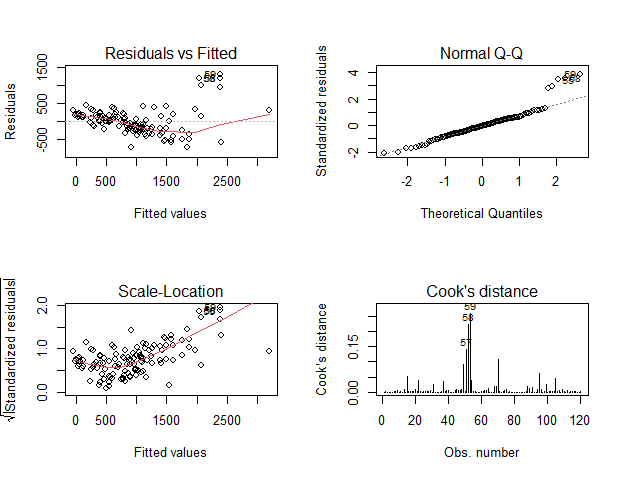
\includegraphics[width=13cm]{diagnosticGraphs.png}
	\caption{Diagnostični grafi za preverjanje ustreznosti modela}
	\label{figure:3}
\end{figure}

Zgornji levi graf (Residuals vs Fitted) preverja linearnost modela. Prikazuje
ostanke $ \epsilon_{i} $ v odvisnosti od predvidenih vrednosti. Če točke
izgledajo naključno razporejene, pomeni da so napake nalkjučno razporejene in
naš model je ustrezen. Točke za naš model pa imajo neko zvezo, na prvi pogled
izgleda negativno linearna. To pomeni, da v našem modelu manjka neka funkcija,
ki bi te napake odpravila. Naš model zato ni najboljši in bi se ga dalo
izboljšati.

Zgornji desni graf (Normal Q-Q) prikazuje normalnost porazdelitve
standardiziranih ostankov. Če točke tvorijo premico, lahko sklepamo, da so
napake normalno porazdeljene in naš model je v redu. Ker točke na desni strani
zelo odstopajo od premice, napake ne izgledajo normalno porazdeljene. To
dodatno potrdi rezultat ukaza {\sf shapiro.test(model\$residuals)}, ki hipotezo
o normalnosti ovrže z w vrednostjo $ 0.91457 $ in s p vrednostjo $ 1.18e-06 $.

Spodnji levi graf (Scale-Location) predstavlja varianco napak glede na
predvidene vrednosti. Če je model dober, je varianca napak konstantna.
Na grafu varianca napak ni konstantna in sledi neki polinomski funkciji.
To potrjuje tudi Breusch-Pagan-ov test, ki testira hipotezo o konstantnosti
napak proti hipotezi, da napake niso konstantne. Kličemo ga s funkcijo
{\sf ncvTest(model)}. Za naš model dobimo p vrednost manjšo od $ 2.22e-16 $,
kar pomeni, da ovržemo hipotezo o konstantnosti napak.

Spodnji desni graf (Cook's distance) prikazuje, kateri podatki najbolj
vplivajo na model. Cook-ova razdalja se izračuna tako, da se za vsak podatek
izračuna model z njim in brez njega. Razlika med vsemi razlikami teh dveh
modelov je Cook-ova razdalja posameznega podatka. Če je razdalja velika,
to pomeni, da podatek močno vpliva na model. Če je tak podatek neobičajen in
izstopa med drugimi podatki, ga lahko poskusimo odstraniti. Druga možnost pa
je, da našim podatkom ustreza nek drugi model, ki bolje opisuje zvezo med
neodvisnimi spremenljivkami in odvisno spremenljivko. Za naš primer lahko točke
s preveliko razdaljo dobimo z ukazom {\sf points $\leftarrow$ which(cooks.distance(model) $ > $ 4/118)}.
Ali ima neka točka prevelik vpliv, lahko izračunamo z ukazom
{\sf any(cooks.distance(fit)[points] $ > $= qf(0.5, 4, 118))}. Ukaz vrne FALSE,
kar pomeni, da ne rabimo odstraniti nobene točke iz naših podatkov.

Za koeficiente našega modela pa lahko tudi izračunamo intervale zaupanja za
$ 95\% $ gotovost. Intervale za vsak koeficient dobimo z ukazom {\sf confint(model)}, ki
nam vrne naslednjo tabelo:
\begin{table}[H]
\begin{center}
\caption{Intervali zaupanja koeficientov spremenljivk}
\begin{tabular}{ c|cc }
	& 2.5\% & 97.5\% \\
	\hline
	(Intercept) & -12011.4967 & -2937.7897 \\
	letoGradnje & 1.5365 & 6.1651 \\
	povrsina & 13.6955 & 17.1995 \\
	oddaljenost & -139.6602 & -5.7400 \\
	parkirisce & -333.0987 & -48.2166 \\
\end{tabular}
\end{center}
\end{table}
Intervali zaupanja so za vse koeficiente precej veliki, zato naš model ni
ustrezen. K velikosti intervalov prispeva standardna napaka posameznih
spremenljivk modela, ki jih dobimo pod {\sf Std. Error} pri izpisu ukaza
\ref{lst:1}.

\subsection{Predlogi izboljšave modela}

Linearni model se ni izkazal za najboljši opis mojih podatkov, zato sem
poskusil še z linearno kombinacijo nelinearnih funkcij spremenljivk.
Izračunal sem še kvadratno, korensko, logaritemsko in ekspomentno funkcijo
za spremenljvke $ letoGradnje, povrsina $ in $ oddaljenost $. Spremenljivke
$ parkirisce $ se nisem dotikal, saj je diskretna in zavzame samo dve
vrednosti.

Najprej sem z ukazom {\sf lm} preveril regresijski model za kar vse prej
naštete spremenljivke. Ta model pravi, da na najemnino vplivata samo člena
$ e^{povrsina} $ in $ povrsina^{2} $ s p vrednostima $ 0.00483 $ in $ 0.03561 $.
Pri vseh ostalih členih drži ničelna hipoteza linearne regresije, in sicer, da
so njihovi koeficienti enaki $ 0 $. Model tudi pojasni $ 80.25\% $ variabilnosti
cene, kar je za $ 5.81\% $ bolje kot prejšnji model, vendar ima še vedno vse
pomankljivosti prejšnjega modela. Ta rezultat pa nam pove, da je mesečna
najemnina po vsej verjetnosti polinomska funkcija površine stanovanja.

Izračunal sem še nekaj potenčnih vrednosti površine in preveril model samo za
ceno v odvisnosti od polinoma površine. Tokrat se je izkazalo, da so vsi členi
polinoma obdržali ničelno hipotezo, da so njihovi koeficienti enaki $ 0 $. Iz
tega lahko sklepamo, da tudi druge spremenljivke vplivajo na mesečno najemnino,
saj površina sama ne more opisati cene najemnine.

Preveril sem še nekaj linearnih kombinacij raznih funkcij spremenljivk, vendar
nisem našel ustrezne kombinacije, ki bi zadoščala predpostavkam regresijskega
modela. Zato sem se odločil še malo pogledati podatke.

Iz grafa preverjanja linearnosti modela iz slike \ref{figure:3}
(Residuals vs Fitted) lahko vidimo, da napake padajo z višjo najemnino, torej
je model napovedal višje cene za dražja stanovanja, kot pa dejansko so,
najdražja stanovanja pa je ocenil z nižjo ceno od dejanske. Če iz podatkov
odstranim stanovanja dražja od 1500€ in poskusimo ponovno določiti regresijski
model, dobimo dober model za stanovanja, cenejša od 1500€. Standardna napaka
novega modela za cenejša stanovanja je samo $ 144 $, kar je veliko manj od
prvotnega modela. Prirejeni $ R^{2} = 76.14\% $, kar je za samo $ 1.7\% $ bolje
od prejšnjega modela. Prav tako so za ta model izpolnjeni vsi pogoji
regresijskega modela. Napake so porazdeljene normalno, prav tako so konstantne
variance napak in nobene točke ni potrebno odstraniti iz modela. Formula modela
za stanovanja, cenejša od 1500€, je naslednja:
\begin{equation}
\begin{split}
	skCena = &-3025.2037+1.7112*letoGradnje \\
			&+8.3316*povrsina-53.7657*oddaljenost+\epsilon
\end{split}
\end{equation}
Pri tem pa je treba vedeti in paziti, da smo odstranili $ 17 $ najdražjih
stanovanj, zato modela med sabo nista enakovredna, saj opisujeta druge
podatke. Ta model pa nakazuje na to, da obstajajo različni modeli opisa
najemnine glede na cenovni rang mesečne najemnine.

\section{Zaključek}

Ugotovil sem, da je cena mesečne najemnine odvisna predvsem od površine
stanovanja, ki ga najemamo. Model opisa cene najemnine pa ni najboljši, saj
pojasni $ 74.44\% $ variance cene najema, prav tako pa so napake razporejene
nenaključno, kar nakazuje na mankajočo funkcijo v modelu opisa. Prav tako je
možno, da v modelu manjka neka neznana zvezna spremenljivka. Ugotovil sem tudi,
da je možno, da obstajata dva modela opisa najemnine stanovanj, eden za
luksuzna in drugi za neluksuzna stanovanja. Na to me napeljuje dejstvo, da sem
dobil veliko boljši opisni model po odstranitvi stanovanj, ki so imela
najemnino 1500€ in več.

\section{Literatura}

[0]
https://www.distance.to/

[1] Analiza dejavnikov oglaševanih cen rabljenih stanovanj v Ljubljani in njeni
okolici, Sonja Friškovec, Aleksander Janeš, Univerza na Primorskem, jesen 2010

[2] Dejavniki oblikovanja prodajnih cen stanovanj, Mojca Repič, Ljubljana,
oktober 2014

[3] \href{https://www.researchgate.net/publication/239329925_A_New_Test_of_Symmetry_about_an_Unknown_Median}
enačba 11

[4] \href{https://gitlab.com/ul-fri/ovs/projekt/-/blob/master/regresija.pdf}{A}

\end{document}